Rhythmobox jest podstawowym odtwarzaczem muzyki w systemie Ubuntu. Dwukrotne kliknięcie na plik dźwiękowy otwiera odtwarzacz i rozpoczyna odtwarzanie wybranego pliku audio. Otworzenie w menadżerze plików wielu plików dźwiękowych na raz uruchamia Rhythmboxa i ustawia wszystkie wybrane pliki w kolejce odtwarzania.

Rhythmobox korzysta z zainstalowanych w systemie kodeków. jeżeli zgodnie z tym przewodnikiem zainstalowałem pakiet \textcolor{ubuntu_orange}{ubuntu-restricted-extras} to Rhythmobox będzie wstanie odtworzyć każdy popularny format audio.
\begin{center}
	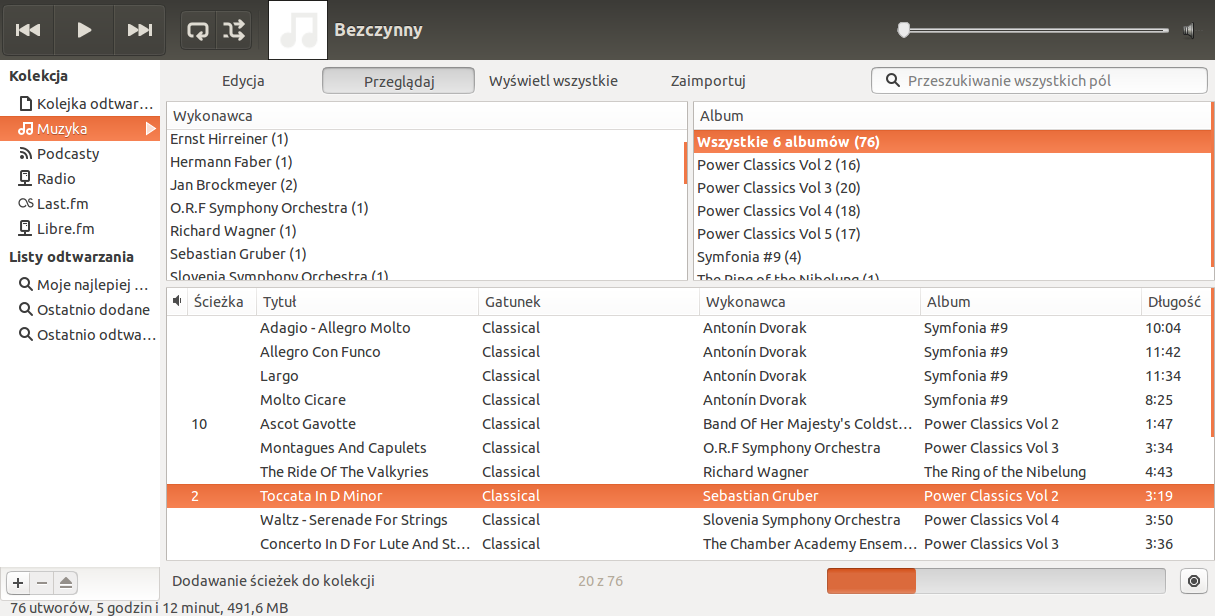
\includegraphics[width=\linewidth]{images/programy_rhythmbox1.png}
\end{center}

\subsubsection{Podstawy obsługi programu Rhythmbox}
\begin{wrapfigure}{r}{0.5\textwidth}
                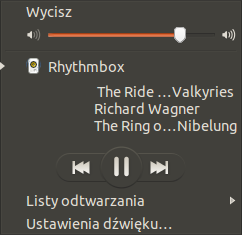
\includegraphics[width=\linewidth]{images/programy_rhythmbox2.png}
\end{wrapfigure}

W systemowym menu dźwięk 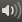
\includegraphics{images/ikony_dzwiek.png} możesz uruchomić i sterować Rhythmboxem (oraz innymi odtwarzaczami muzyki, jeżeli masz je zainstalowane). W tym menu wyświetlane są informacje o aktualnie odtwarzanym utworze oraz przyciski sterujące pozwalające sterować odtwarzaczem muzyki, wgrywać listy odtwarzania itp.

Kolekcja:
\begin{itemize}
\item Wszystkie pliki audio znajdujące się w katalogu Muzyka, znajdującym się w Twoim katalogu domowym, są automatycznie dodawane do kolekcji.
\item Aby wskazać inne katalogi wybierz \menu{{Modyfikuj}>{Preferencje}>{Muzyka}>{Pliki muzyczne znajdują się w:}} i wskaż, który katalog program ma obserwować.
\item Wybierz \textcolor{ubuntu_orange}{Zaimportuj} w głównym oknie programu i wskaż katalog.
\end{itemize}
Odsłuchiwanie muzyki:
\begin{itemize}
\item Dwukrotne kliknięcie na plik w głównym oknie programu rozpoczyna jego odtwarzanie. Po zakończeniu odtwarzania Rhythmbox rozpocznie odtwarzanie koljnego utworu z listy.
\item Zamknięcie okna programu nie powoduje przerwania jego pracy. Rhythmbox może działać w tle i być sterowany za pośrednictwem ikony dźwięku 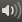
\includegraphics{images/ikony_dzwiek.png} na pasku menu.
\end{itemize}
Tworzenie kolejki odtwarzania:
\begin{enumerate}
\item Zaznacz jeden lub więcej utworów. Trzymając wciśnięty klawisz \keys{Shift} możesz zaznaczyć wiele kolejnych utworów. Trzymając wciśnięty klawisz \keys{CTRL} możesz kilknięciami myszy wybrać poszczególne utwory.
\item Kliknij i przytrzymaj wciśnięty lewy klawisz myszy a następnie przesuń zaznaczone utwory na pozycję \textcolor{ubuntu_orange}{Kolejka odtwarzania} znajdującą się w panelu po lewej.
\item Alternatywnie kliknij prawym przyciskiem myszy i wybierz z menu kontekstowego \textcolor{ubuntu_orange}{Dodaj do kolejki}.
\end{enumerate}
Tworzenie listy odtwarzania:
\begin{enumerate}
\item Zaznacz jeden lub więcej utworów. Trzymając wciśnięty klawisz \keys{Shift} możesz zaznaczyć wiele kolejnych utworów. Trzymając wciśnięty klawisz \keys{CTRL} możesz kilknięciami myszy wybrać poszczególne utwory.
\item  Kliknij prawym przyciskiem myszy na zaznaczone utwory i z menu kontekstowego wybierz \textcolor{ubuntu_orange}{Dodaj do listy odtwarzania}.
\begin{itemize}
\item \menu{{Dodaj no nowej listy odtwarzania}} utworzy nową listę odtwarzania. Pojawi się ona w panelu po lewej stronie okna. Klikając na nową listę możesz zmienić jej nazwę.
\item Jeżeli masz już własne listy odtwarzania to w tym menu możesz dodać do nich nowe utwory.
\end{itemize}
\end{enumerate}